\chapter{}

\section{引言}

\begin{figure}[!htbp]
    \centering
    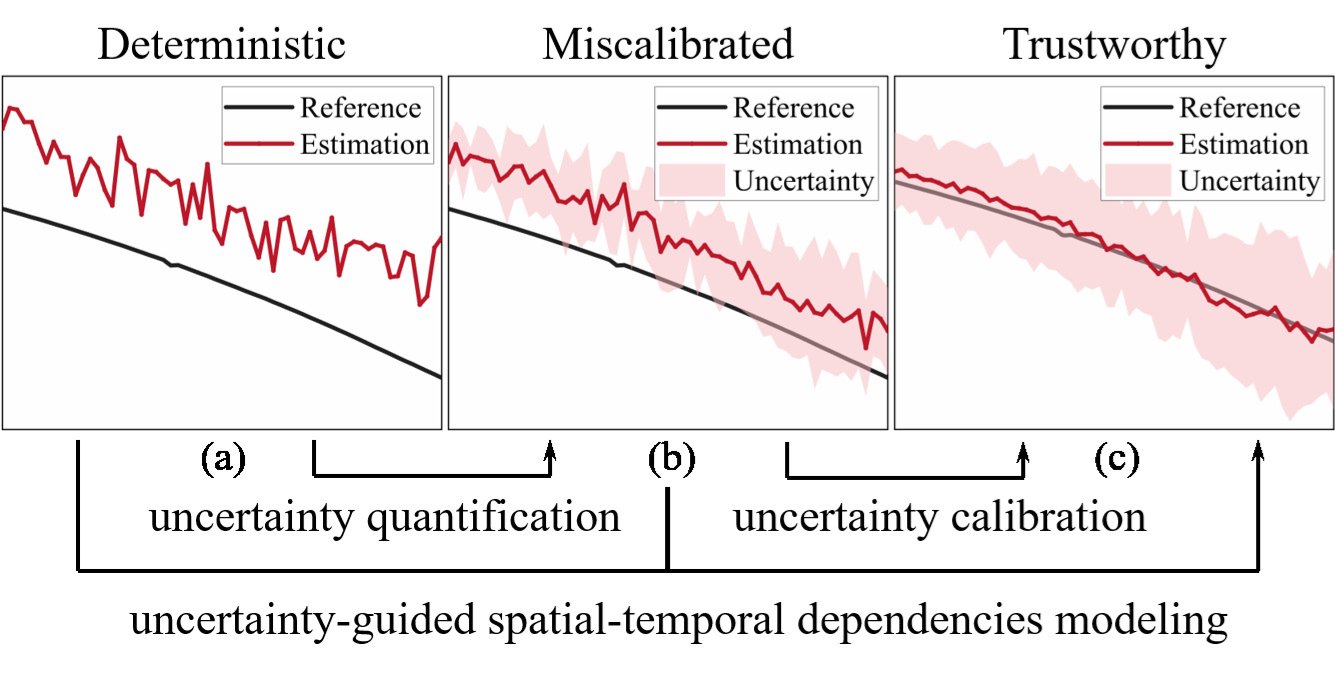
\includegraphics[width=\textwidth]{Img/HSSTT_figures/trans/FIG1_TII-25-2632.pdf}
    \bicaption{挑战}{challenges}
    \label{fig:hsstt_challenges}
\end{figure}

\section{锂离子电池健康状态估计方法}

\begin{figure}[!htbp]
    \centering
    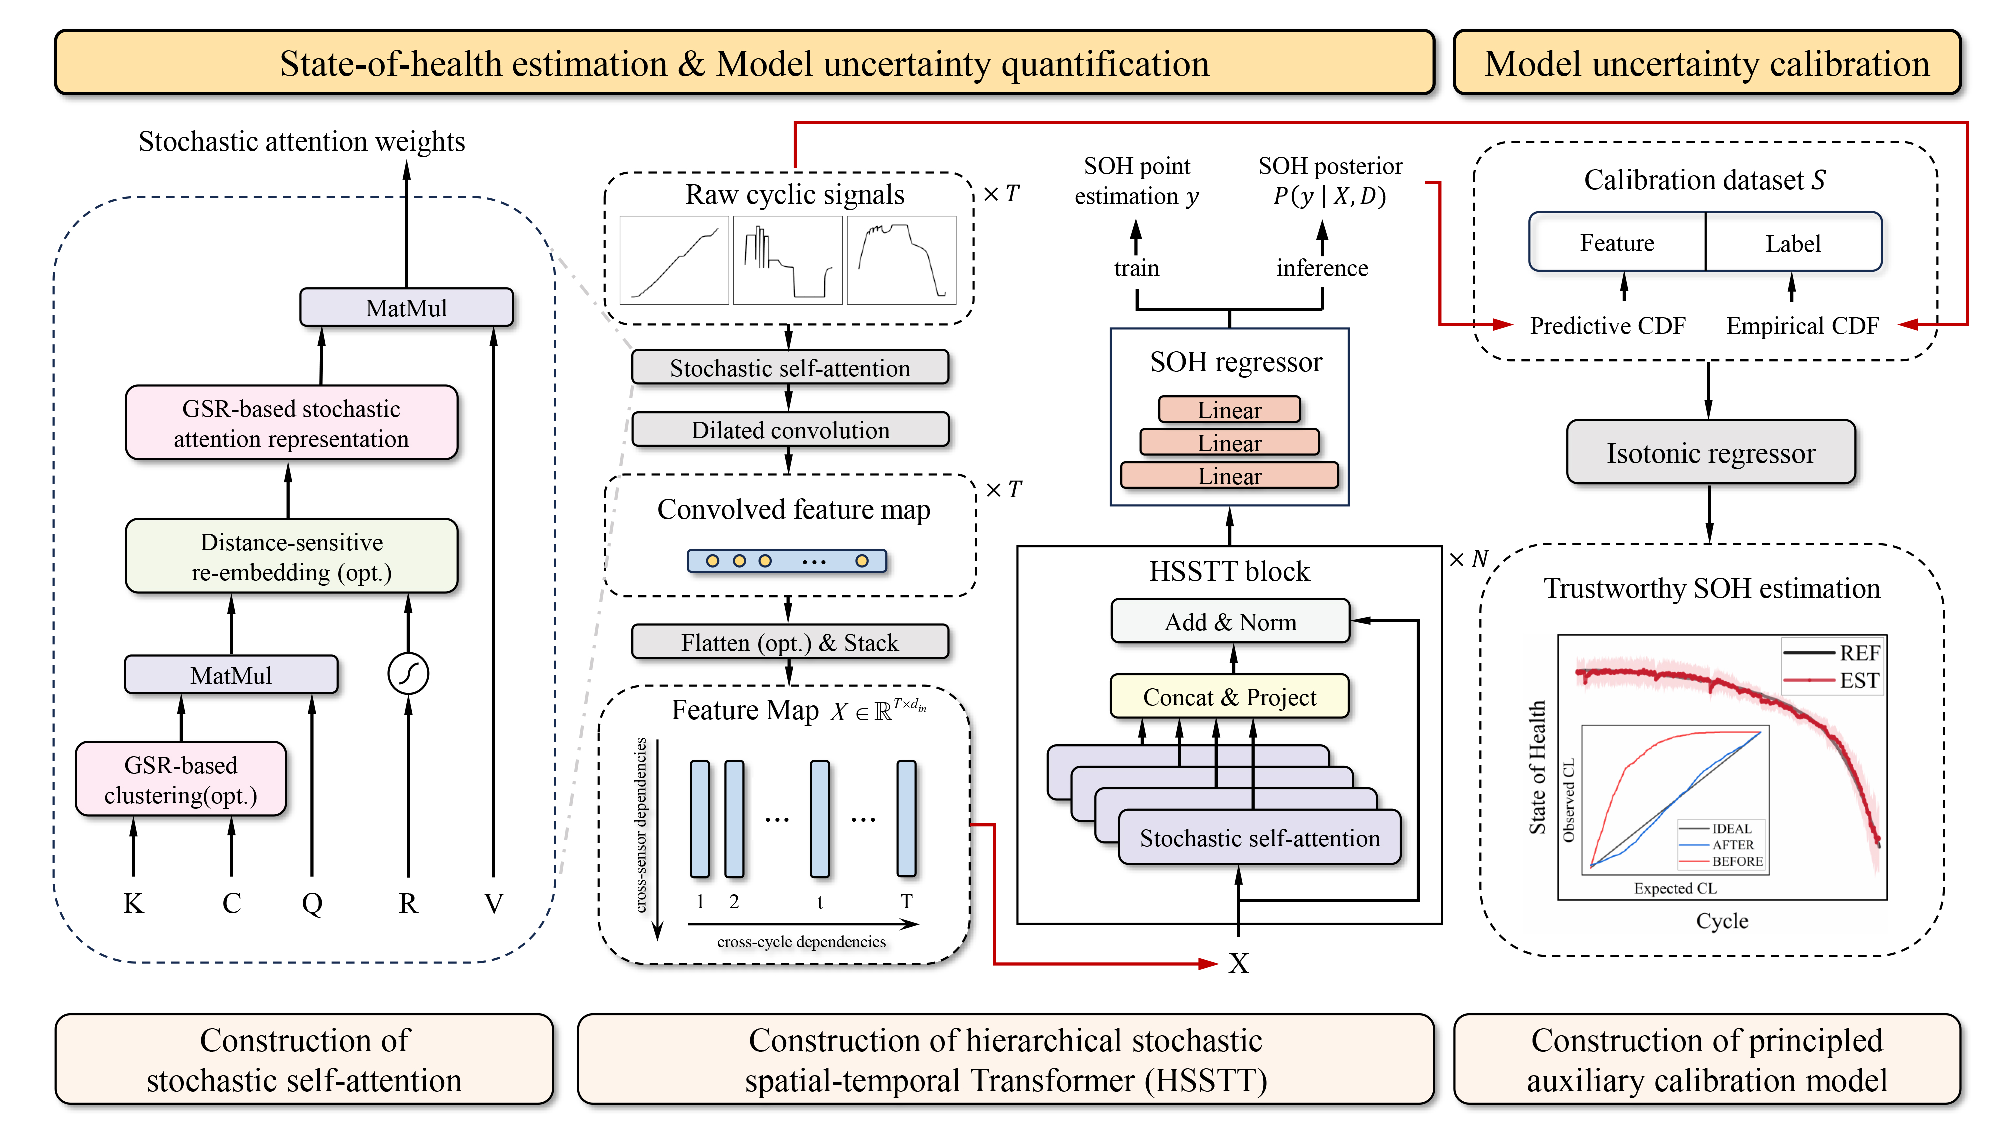
\includegraphics[width=\textwidth]{Img/HSSTT_figures/trans/FIG2_TII-25-2632.pdf}
    \bicaption{HSSTT~架构图}{Diagram of the HSSTT framework}
    \label{fig:hsstt_framework}
\end{figure}

Lin等\cite{9729404}

\section{实验评估}

\subsection{实验设置}

\subsection{性能对比实验}

\begin{figure}[!htbp]
    \centering
    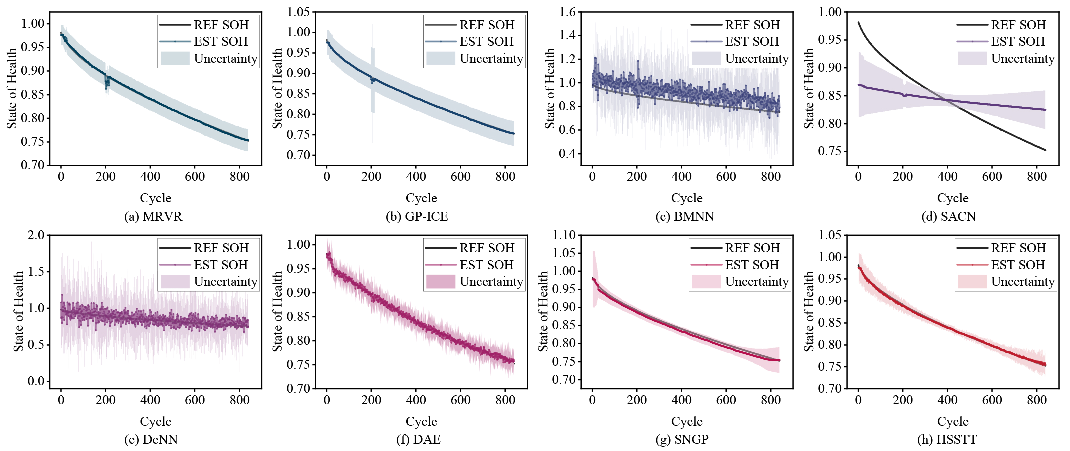
\includegraphics[width=\textwidth]{Img/HSSTT_figures/trans/FIG3_TII-25-2632.pdf}
    \bicaption{HSSTT~架构图}{Diagram of the HSSTT framework}
    \label{fig:hsstt_comparison}
\end{figure}

\begin{figure}[!htbp]
    \centering
    \includegraphics[width=\textwidth]{Img/HSSTT_figures/trans/FIG4_TII-25-2632.pdf}
    \bicaption{HSSTT~架构图}{Diagram of the HSSTT framework}
    \label{fig:hsstt_efficiency}
\end{figure}

\subsection{消融实验}

\begin{figure}[!htbp]
    \centering
    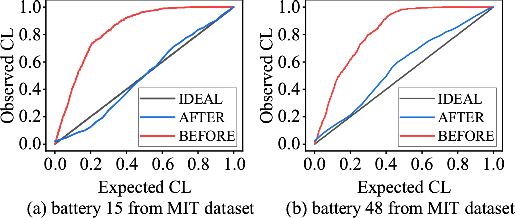
\includegraphics[width=\textwidth]{Img/HSSTT_figures/trans/FIG5_TII-25-2632.pdf}
    \bicaption{HSSTT~架构图}{Diagram of the HSSTT framework}
    \label{fig:hsstt_ablation}
\end{figure}

\subsection{超参数敏感性分析}

\begin{figure}[!htbp]
    \centering
    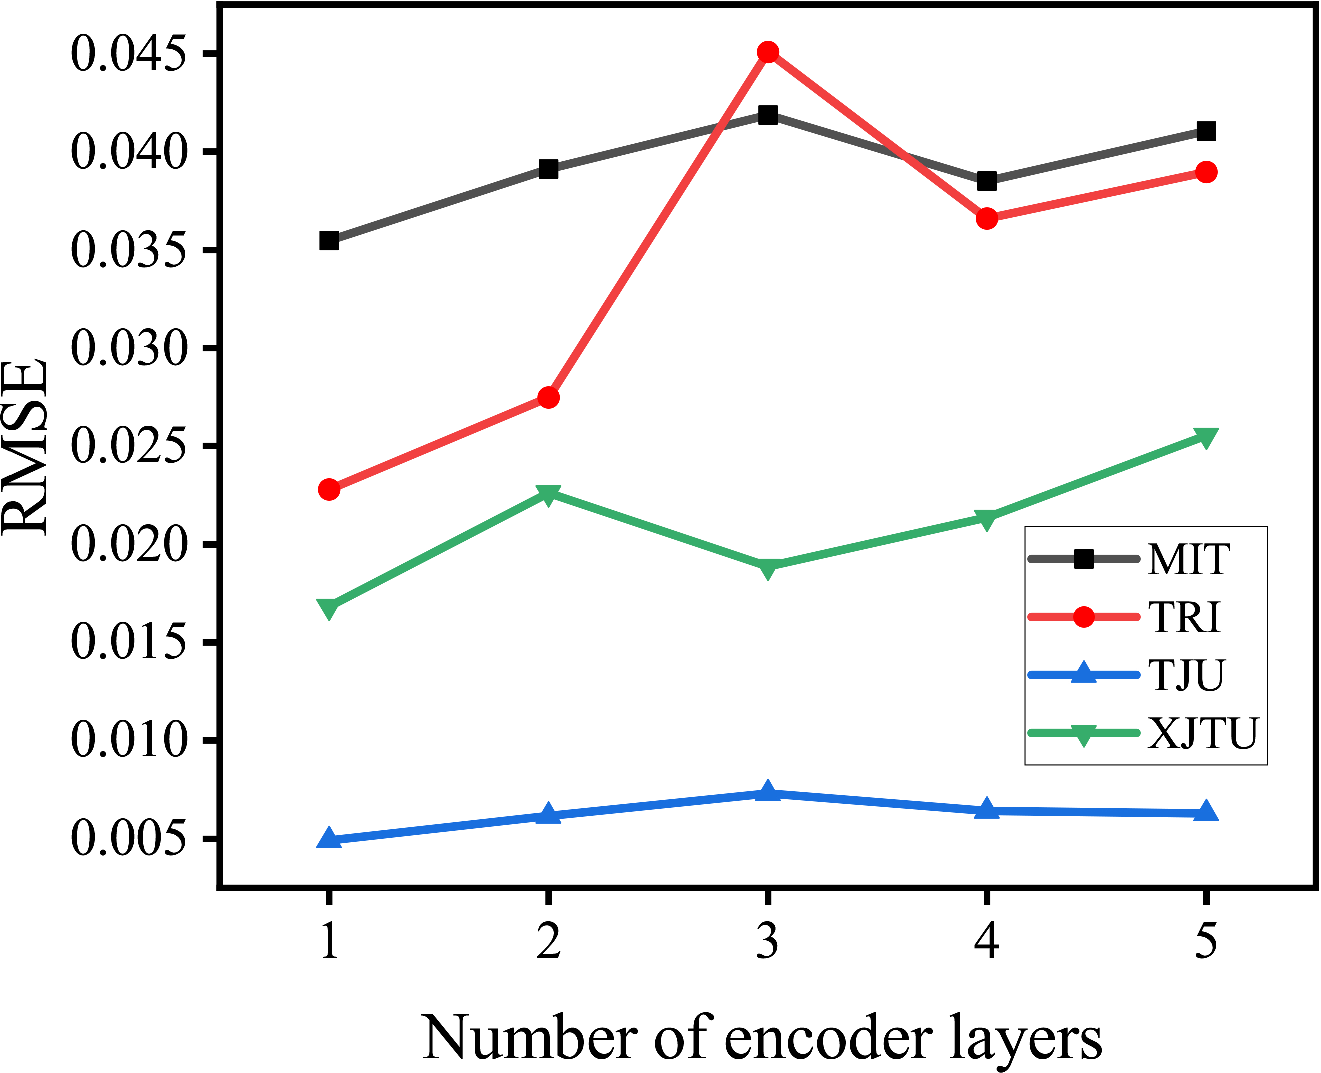
\includegraphics[width=\textwidth]{Img/HSSTT_figures/trans/FIG6a_TII-25-2632.pdf}
    \bicaption{HSSTT~架构图}{Diagram of the HSSTT framework}
    \label{fig:hsstt_sensitivity_el}
\end{figure}

\begin{figure}[!htbp]
    \centering
    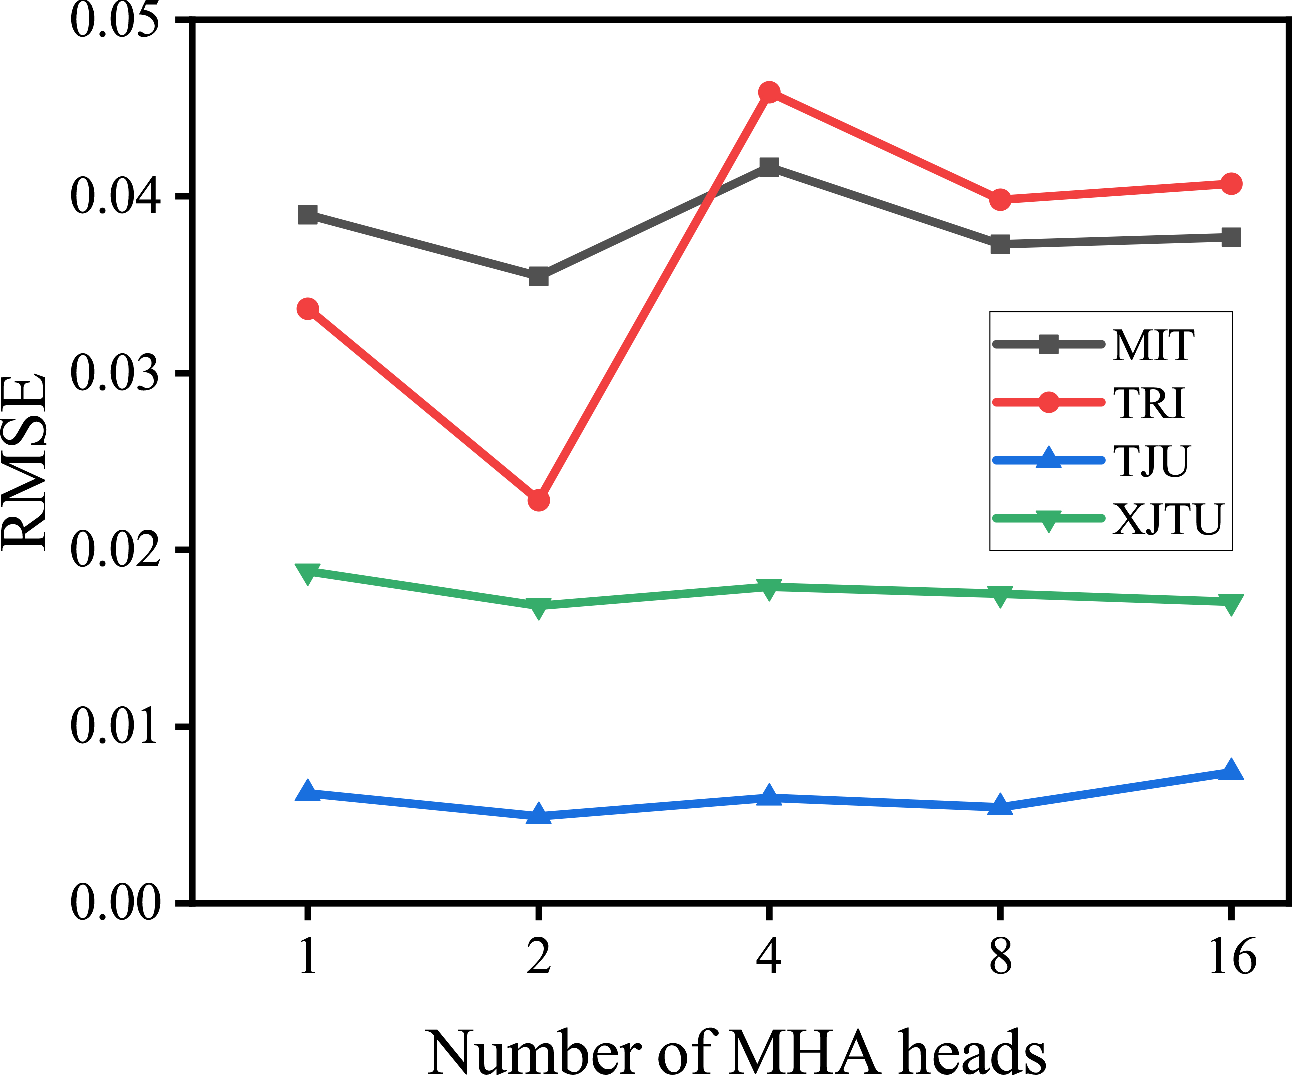
\includegraphics[width=\textwidth]{Img/HSSTT_figures/trans/FIG6b_TII-25-2632.pdf}
    \bicaption{HSSTT~架构图}{Diagram of the HSSTT framework}
    \label{fig:hsstt_sensitivity_nh}
\end{figure}

\begin{figure}[!htbp]
    \centering
    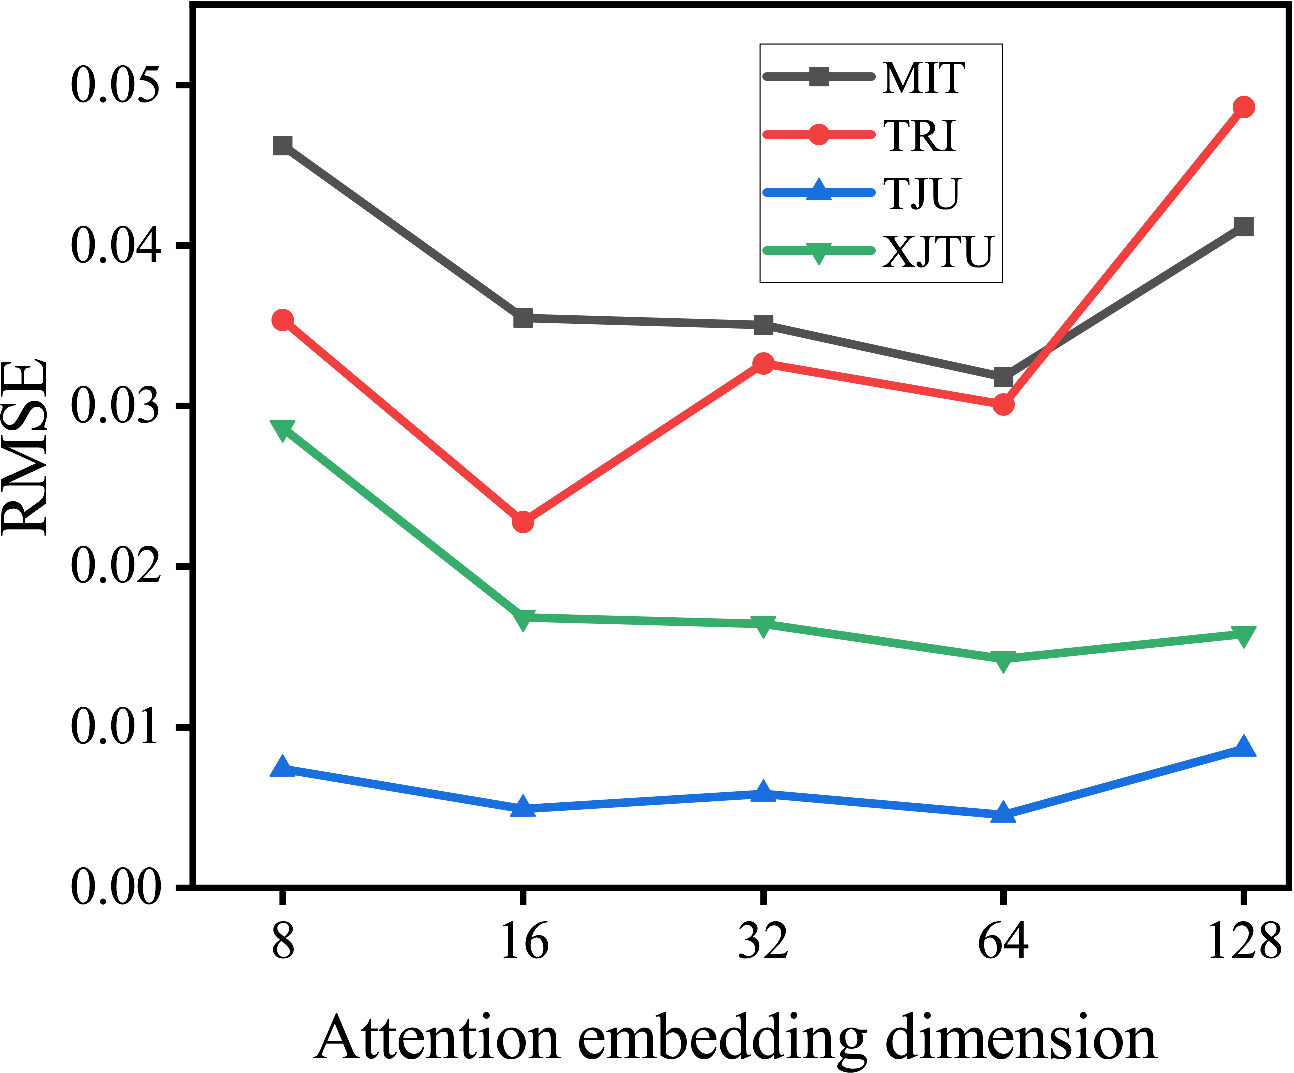
\includegraphics[width=\textwidth]{Img/HSSTT_figures/trans/FIG6c_TII-25-2632.pdf}
    \bicaption{HSSTT~架构图}{Diagram of the HSSTT framework}
    \label{fig:hsstt_sensitivity_ed}
\end{figure}

\begin{figure}[!htbp]
    \centering
    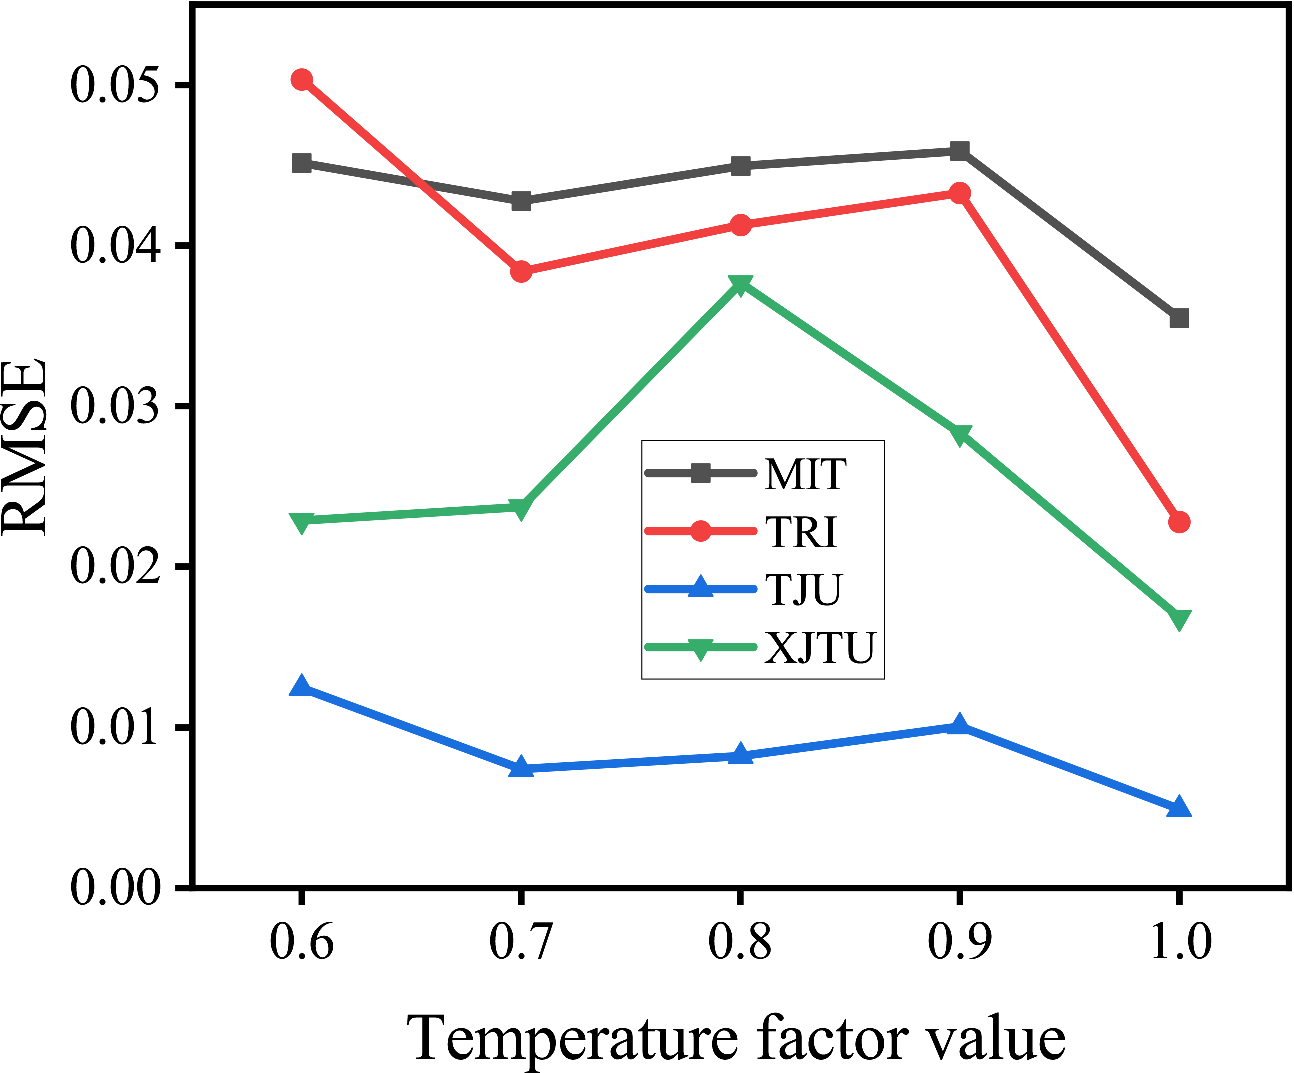
\includegraphics[width=\textwidth]{Img/HSSTT_figures/trans/FIG6d_TII-25-2632.pdf}
    \bicaption{HSSTT~架构图}{Diagram of the HSSTT framework}
    \label{fig:hsstt_sensitivity_tf}
\end{figure}

\subsection{分布内外退化模式辨识实验}

\begin{figure}[!htbp]
    \centering
    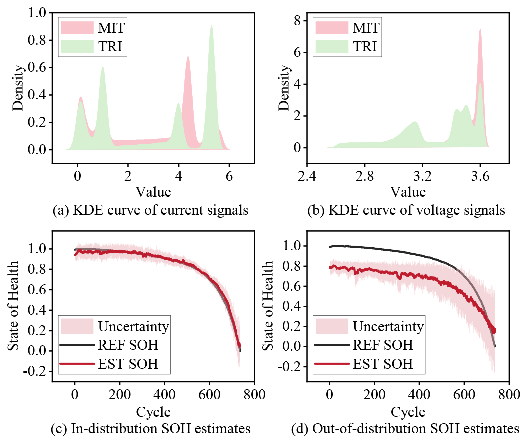
\includegraphics[width=\textwidth]{Img/HSSTT_figures/trans/FIG7_TII-25-2632.pdf}
    \bicaption{HSSTT~架构图}{Diagram of the HSSTT framework}
    \label{fig:hsstt_sensitivity_ood}
\end{figure}

\section{本章小结}